\documentclass{standalone}
\usepackage{amsmath,amsfonts,amssymb}
\usepackage{tikz,pgfplots}
\usetikzlibrary{arrows,arrows.meta,bending,calc,decorations,shadings,shadows,shapes,shapes.arrows,shapes.geometric}
\usetikzlibrary{calc,fadings,decorations.pathreplacing}
\usepgfplotslibrary{units,fillbetween,groupplots,colorbrewer}
\usetikzlibrary{pgfplots.colorbrewer,}
\usepackage{pgfplotstable}

\pgfdeclareplotmark{*)}
{\shade[draw=red!60!black,ball color=red!70,opacity=0.5] (0,0) circle [radius=2pt];}


\newcommand*{\xMin}{0.2}%
\newcommand*{\xMax}{11}%
\newcommand*{\yMin}{0}%
\newcommand*{\yMax}{5}%

\begin{document}
	
	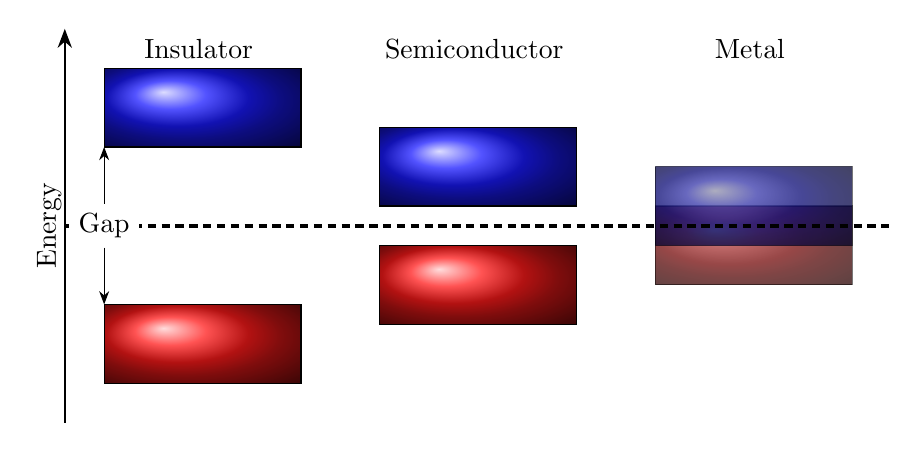
\begin{tikzpicture}
		
%		\draw[step=.5cm,gray,very thin,opacity=0.1] (0.2,0) grid (11cm,5cm);
%		 \foreach \i in {\xMin,...,\xMax} {
%			\draw [very thin,gray] (\i,\yMin) -- (\i,\yMax)  node [below] at (\i,\yMin) {$\i$};
%		}
%		\foreach \i in {\yMin,...,\yMax} {
%			\draw [very thin,gray] (\xMin,\i) -- (\xMax,\i) node [left] at (\xMin,\i) {$\i$};
%		}
%	
	
	\draw[-{Stealth},line width=0.3mm] (0.5,0)-- node[midway,rotate=90, yshift=2mm] {Energy}(0.5,5);
	
		\node at (2.2,4.75) {Insulator};
    	\filldraw[ball color=red!90!white] (1,0.5) rectangle (3.5,1.5);
		\filldraw[ball color=blue!90!white] (1,3.5) rectangle (3.5,4.5);
		
		\node at (5.7,4.75) {Semiconductor};
		\filldraw[ball color=blue!90!white] (4.5,2.75) rectangle (7,3.75);
		\filldraw[ball color=red!90!white] (4.5,1.25) rectangle (7,2.25);
		
		\node at (9.2,4.75) {Metal};
		\filldraw[ball color=red!90!white,opacity=0.5] (8,1.75) rectangle (10.5,2.75);
		\filldraw[ball color=blue!90!white,opacity=0.5](8,2.25) rectangle (10.5,3.25);
		
		
		\draw[densely dashed, line width=0.5mm](0.5,2.5)--(11,2.5);
		
		
		
		
		\node[fill=white] (point) at (1,2.5) {Gap};
		\draw[-Stealth] (point) -- (1,1.5);
		\draw[-Stealth] (point) -- (1,3.5);
		%\draw[{Stealth[scale=1]}-,line width=0.7pt]   (point) --  (1,1.5);
	\end{tikzpicture}
	
	
	
\end{document}